
\documentclass[12pt]{article}

% Package lists
\usepackage{listings}
\usepackage{xcolor}
\usepackage{geometry}
\usepackage{enumitem}
\usepackage{graphicx}
\usepackage{mathtools}

% Configurations here
\DeclarePairedDelimiter\ceil{\lceil}{\rceil}
\definecolor{codegreen}{rgb}{0,0.6,0}
\definecolor{codegray}{rgb}{0.5,0.5,0.5}
\definecolor{codepurple}{rgb}{0.58,0,0.82}
\definecolor{backcolour}{rgb}{0.95,0.95,0.92}
 
\lstdefinestyle{mystyle}{
    backgroundcolor=\color{backcolour},   
    commentstyle=\color{codegreen},
    keywordstyle=\color{magenta},
    numberstyle=\tiny\color{codegray},
    stringstyle=\color{codepurple},
    basicstyle=\ttfamily\footnotesize,
    breakatwhitespace=false,         
    breaklines=true,                 
    captionpos=b,                    
    keepspaces=true,                 
    numbers=left,                    
    numbersep=5pt,                  
    showspaces=false,                
    showstringspaces=false,
    showtabs=false,                  
    tabsize=2
}
\lstset{style=mystyle}

\geometry{margin=1cm, bottom=2cm}
\setlength{\columnseprule}{1pt}

\begin{document}
  \title{Last Homework - Discrete Mathematics}
  \author{Nguyen Tien Duc - ITITIU18029}
  \maketitle

  \part*{10.1}
    \section*{4}
      \begin{enumerate}[label=\alph*)]
        \item Vertice a is the root
        \item Internal vertices: a, b, d, e, g, h, i, o
        \item Leaves vertices: c, f, j, k, l, m, n, q, r, s, p
        \item j has no children vertice.
        \item Sibling of o: p
        \item Ancestor of m: g, b, a
        \item Descendants of b: e, f, g, j, k, l, m
      \end{enumerate}
    \section*{6}
      Some vertices have 3 children, while some only have 1 or 2 children. Therefore, that is not a full m-ary tree.
    \section*{10}
      \begin{center}
        \begin{tabular}{ccc}
          a)
          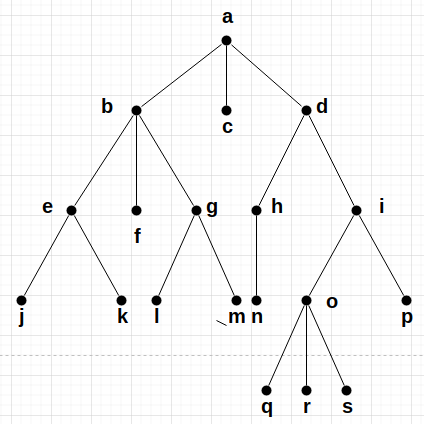
\includegraphics{10_a.png} 
          & 
          b)
          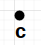
\includegraphics{10_c.png} 
          & 
          c)
          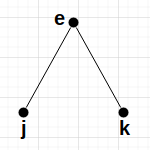
\includegraphics{10_e.png} 
        \end{tabular}
      \end{center}
    \section*{22}
      The model is a full 5-ary tree with 10,000 internal vertices. \\
      Total number of vertices: \(n = m \cdot i + 1 = 5 \cdot 10,000 + 1 = 50,001 \) vertices \\
      All vertices except the root received the letter. Thus, there are 50,000 people received the letter.\\
      Leaves vertices represent people who received but did not send out the letter. Thus, the number of people in this group is: 50,001 - 10,000 = 40.001 people.
    \section*{28}
      \begin{center}
        A full m-ary tree of height h has:\\
        \(m^0\) vertices at level 0. \\
        \(m^1\) vertices at level 1. \\
        \(m^2\) vertices at level 2. \\
        \(\dots\)\\
        \(m^h\) vertices at level h. \\
        Therefore, total number of vertices is a geometric series:
        \[n = m^0 + m^1 + m^2 + \dots + m^h = \frac{m^{h+1}-1}{m-1}\]
        Number of leaves is the number of vertices at level h: \(m^h\)
      \end{center}

    \section*{32}
      The root of the tree represents the entire book.\\
      The vertices at level 1 represents chapters of the book.\\
      The vertices at level 2 represents sections of the book.\\
      The vertices at level 3 represents subsections of the book.
  \part*{10.2}
    \section*{2}
      \begin{center}
        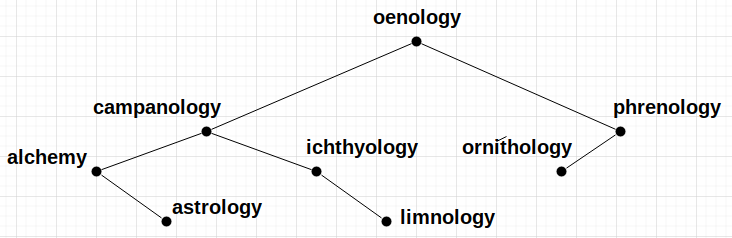
\includegraphics{binary-search.png}
      \end{center}
    \section*{6}
      1 counterfeit coin in 4 coins. Thus, there are 4 outcomes corresponding to 4 leaves.\\
      Each comparison has 3 outcomes, corresponding to a tinary tree.\\
      Therefore, \(h \geq \ceil*{log_34} = 2\)\\
      \(\Rightarrow\) At least 2 weighings are needed.\\
      Algorithm using 2 comparisons: 
      \begin{itemize}
        \item Divide 4 coins into 2 groups and compare the total weight of 2 groups. The light group contains the counterfeit coin.
        \item Compare 2 coins in the group that contains the counterfeit coin. The lighter coin is the counterfeit one.
      \end{itemize}  
    \section*{20}
      \begin{center}
        \begin{tabular}{ccc}
          a)
          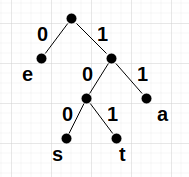
\includegraphics{20_a.png} 
          & 
          b)
          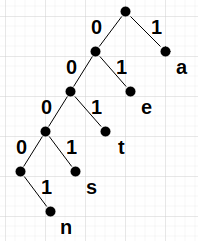
\includegraphics{20_b.png} 
          & 
          c)
          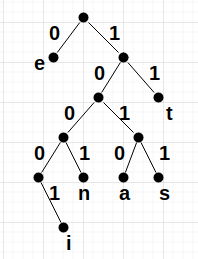
\includegraphics{20_c.png} 
        \end{tabular}
      \end{center}
    \section*{22}
      \begin{tabular}{cccc}
        a) test & b) beer & c) sex & d) tax
      \end{tabular}
  \part*{10.3}
    \section*{4}
      \begin{enumerate}[label=\alph*)]
        \item Level 5
        \item Address of parent of v: 3.4.5.2
        \item v has at least 3 siblings
        \item T has at least 1 root node and 3 + 4 + 5 + 2 + 4 internal nodes, totally 19 vertices.
        \item Other addresses that must occur: o, 1, 2, 3, 3.1, 3.2, 3.3, 3.4, 3.4.1, 3.4.2, 3.4.3, 3.4.4, 3.4.5, 3.4.5.1, 3.4.5.2, 3.4.5.2.1, 3.4.5.2.2, 3.4.5.2.3
      \end{enumerate}
    \section*{8}
      Preorder traversal: a, b, d, e, i, j, m, n, o, c, f, g, h, k, l, p
    \section*{12}
      Inorder traversal: k, e, l, m, b, f, r, n, s, g, a, c, o, h, d, i, p, j, q
    \section*{14}
      Postorder traversal: d, i, m, n, o, j, e, b, f, g, k, p, l, h, c, a
    \section*{18}
      \begin{enumerate}[label=\alph*)]
        \item 
          \begin{center}
            \begin{tabular}{cc}
              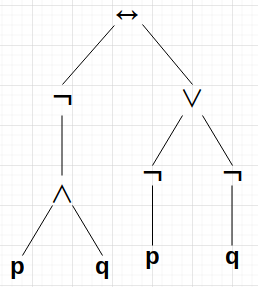
\includegraphics{18a1.png}
              &
              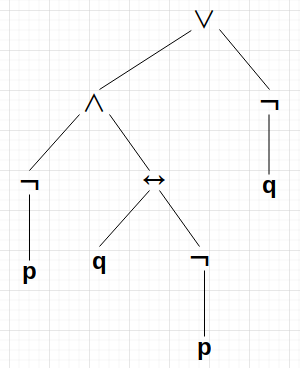
\includegraphics{18a2.png} \\
              \(\neg(p\wedge q)\leftrightarrow(\neg p \vee \neg q)\)
              &
              \((\neg p \wedge (q \leftrightarrow \neg p))\vee \neg q\)
            \end{tabular}
          \end{center}
        \item Prefix: \(\leftrightarrow \neg \wedge p \; q \vee \neg p \; \neg q\) and \(\vee \wedge \neg p \leftrightarrow q \; \neg p \; \neg q\)
        \item Postfix: \(p \; q \wedge \neg \;p \neg \; q \neg \vee \leftrightarrow\) and \(p \; \neg \; q \; p \; \neg \leftrightarrow \wedge \; q \; \neg \; \vee \)
        \item Infix: \(((\neg(p\wedge q))\leftrightarrow((\neg p) \vee (\neg q)))\) and \((((\neg p) \wedge (q \leftrightarrow (\neg p)))\vee (\neg q))\)
      \end{enumerate}
  \part*{10.4}
    \section*{2}
      \begin{center}
      Remove edges b-d and c-e:\\
        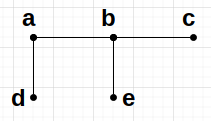
\includegraphics{spanningtree.png}
      \end{center}
    \section*{6}
      \begin{center}
      Remove edges d-e, e-f, f-g, i-j, i-h, i-k, g-h, g-l, k-l, j-l:\\
        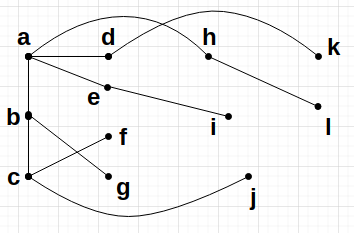
\includegraphics{spanningtree6.png}
      \end{center}
    \section*{10}
      \centering
        Four possible spanning trees:\\
      \begin{tabular}{cc}
        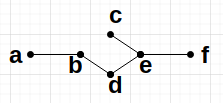
\includegraphics{10-1.png} &
        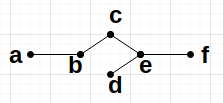
\includegraphics{10-2.png}
        \\
        Remove edge: b-c &
        Remove edge: b-d
        \\
        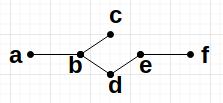
\includegraphics{10-3.png} &
        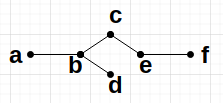
\includegraphics{10-4.png}
        \\
        Remove edge: c-e &
        Remove edge: d-e
      \end{tabular}
\end{document}